\section{Scheduler}\label{sec:Scheduler}
Two tasks are running on the microcontroller, the control algorithm and the communication. The handling of these tasks is however critical. The Vicon system frequency sets a limit for the rate at which the control algorithms can be executed. It is also desirable for the control task to be executed periodically, and at any other time, the microcontroller should listen for new data on the network.

A scheduler can handle priorities and timing of tasks, for this purpose a real time operating system (RTOS) is used, called FreeRTOS \cite{freeRtos}. The capabilities of this RTOS ranges beyond the needs in this project, but provides the necessary tools, and constitutes a flexible base with room for future development.

In \autoref{lst:scheduler} the two main tasks are created with appropriate priorities and the task scheduler is started.

\fxnote{Comment the code}
\begin{lstlisting}[style=customcpp,
                    caption={Code for initialization, creation of the different tasks, start sequence for the motors and call to the scheduler.}, 
                    label=lst:scheduler]
int main()
{
    ... 
    
    ////// Task Creation //////
    //Control Task -> Highest priority
    xTaskCreate(Controllers, "Control", 1000, NULL, configMAX_PRIORITIES - 1, NULL );
    //Communication Task -> High priority but lower than the Control Task
	//	&xHandle for stopping the task if it gets interrupted by the Control Task
    xTaskCreate(Comunication, "Com", 1000, NULL, configMAX_PRIORITIES - 2, &xHandle);
    ...

    ////// Scheduler Start //////
    vTaskStartScheduler();
    return 0;
}
\end{lstlisting}

Once the task scheduler is started the program never returns to main again. The scheduler has a configurable tick-rate, set to \SI{1}{ms}, which it uses to schedule and time tasks. The RTOS is set up to run with preemption, such that the higher priority task, controllers, can preempt the lower priority, communication, in order to achieve a periodic execution of the control algorithms. Since the XBee always sends data out on the RX-pin of the microcontroller, data will be lost if the communication is preempted. To make sure that there is always new data available for each execution of the control task, the execution frequency is chosen low enough such that at least one package is received in each period.\fxnote{make sure that this is still true after the computation time of the control algorithms has grown due to translational controllers}

In \autoref{fig:timingDiagram} a timing diagram is shown, but since package reception is not synchronized with the periodic control task, this is just an example.

\begin{figure}[H]
    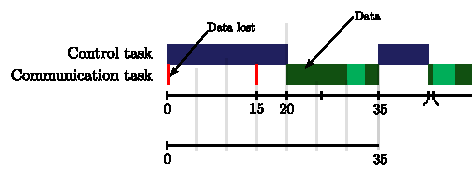
\includegraphics[width =.7\textwidth]{figures/timingDiagram}
    \centering			
    \caption{An example of task execution schedule. The control task is periodic and the packages can arrive at different instances.} 
    \label{fig:timingDiagram}
\end{figure}
\fxnote{Figure under construction - finalize figure when all execution and period times are known. Responsible: Niels}

Although the packages are received at instances unrelated to the control task, the packages still arrive periodically, though the period might fluctuate.